% Options for packages loaded elsewhere
\PassOptionsToPackage{unicode}{hyperref}
\PassOptionsToPackage{hyphens}{url}
%
\documentclass[
]{article}
\usepackage{lmodern}
\usepackage{amssymb,amsmath}
\usepackage{ifxetex,ifluatex}
\ifnum 0\ifxetex 1\fi\ifluatex 1\fi=0 % if pdftex
  \usepackage[T1]{fontenc}
  \usepackage[utf8]{inputenc}
  \usepackage{textcomp} % provide euro and other symbols
\else % if luatex or xetex
  \usepackage{unicode-math}
  \defaultfontfeatures{Scale=MatchLowercase}
  \defaultfontfeatures[\rmfamily]{Ligatures=TeX,Scale=1}
\fi
% Use upquote if available, for straight quotes in verbatim environments
\IfFileExists{upquote.sty}{\usepackage{upquote}}{}
\IfFileExists{microtype.sty}{% use microtype if available
  \usepackage[]{microtype}
  \UseMicrotypeSet[protrusion]{basicmath} % disable protrusion for tt fonts
}{}
\makeatletter
\@ifundefined{KOMAClassName}{% if non-KOMA class
  \IfFileExists{parskip.sty}{%
    \usepackage{parskip}
  }{% else
    \setlength{\parindent}{0pt}
    \setlength{\parskip}{6pt plus 2pt minus 1pt}}
}{% if KOMA class
  \KOMAoptions{parskip=half}}
\makeatother
\usepackage{xcolor}
\IfFileExists{xurl.sty}{\usepackage{xurl}}{} % add URL line breaks if available
\IfFileExists{bookmark.sty}{\usepackage{bookmark}}{\usepackage{hyperref}}
\hypersetup{
  pdftitle={Trabalho Nº3 - Modelos Markovianos},
  pdfauthor={Rafael Morciani \textbar{} GRR20160217},
  hidelinks,
  pdfcreator={LaTeX via pandoc}}
\urlstyle{same} % disable monospaced font for URLs
\usepackage[margin=1in]{geometry}
\usepackage{graphicx,grffile}
\makeatletter
\def\maxwidth{\ifdim\Gin@nat@width>\linewidth\linewidth\else\Gin@nat@width\fi}
\def\maxheight{\ifdim\Gin@nat@height>\textheight\textheight\else\Gin@nat@height\fi}
\makeatother
% Scale images if necessary, so that they will not overflow the page
% margins by default, and it is still possible to overwrite the defaults
% using explicit options in \includegraphics[width, height, ...]{}
\setkeys{Gin}{width=\maxwidth,height=\maxheight,keepaspectratio}
% Set default figure placement to htbp
\makeatletter
\def\fps@figure{htbp}
\makeatother
\setlength{\emergencystretch}{3em} % prevent overfull lines
\providecommand{\tightlist}{%
  \setlength{\itemsep}{0pt}\setlength{\parskip}{0pt}}
\setcounter{secnumdepth}{-\maxdimen} % remove section numbering

\title{Trabalho Nº3 - Modelos Markovianos}
\author{Rafael Morciani \textbar{} GRR20160217}
\date{18 de Agosto de 2020}

\begin{document}
\maketitle

\DeclareUnicodeCharacter{03B3}{$\gamma$}

\hypertarget{exercicio-1---mostrar-que-se-o-estado-x-uxe9-recorrente-e-nuxe3o-se-comunica-com-o-estado-y-entuxe3o-ux3b3_xy0}{%
\subsection{\texorpdfstring{Exercicio 1 - Mostrar que se o estado x é
recorrente e não se comunica com o estado \(y\), então
\(γ_{x,y}=0\)}{Exercicio 1 - Mostrar que se o estado x é recorrente e não se comunica com o estado y, então γ\_\{x,y\}=0}}\label{exercicio-1---mostrar-que-se-o-estado-x-uxe9-recorrente-e-nuxe3o-se-comunica-com-o-estado-y-entuxe3o-ux3b3_xy0}}

\textbf{Desenvolvimento:}

Seja S(x,y) onde \emph{x} é um estado recorrente e não se comunica com
\emph{y}, ou seja, \(\rho_{x,x}=1 \;e \; \rho_{x,y}=0\).

Seja \(C_{n}\) uma cadeia de markov com espaço de estados \emph{S} onde
\(N(y)\) é o número de vezes em que a cadeia permanece no espaço
\emph{y}, então: \[N(y)=\sum_{n=1}^{\infty}l_{y}(C_{n})\]

Também observamos que \(N(y)\geq 1\) é o mesmo que \(T_{y}<\infty\)
logo: \[P_{x}(N(y)\geq1)=P_{x}(T_{y}<\infty)=\rho_{x,y}\] Temos que a
probabilidade com a qual a cadeia começando em \emph{x} visitar a
primeira vez \emph{y} no tempo \emph{m} e visitar novamente no tempo
\emph{n} (onde \emph{m} e \emph{n} são inteiros positivos) é:
\[P_{x}(T_{y}=m).P_{y}(T_{y}=n)\] Logo:
\[P_{x}(N(y)\geq2)=\sum_{m=1}^{\infty}\sum_{n=1}^{\infty}P_{x}(T_{y}=m).P_{y}(T_{y}=n)\\
=\left [ \sum_{m=1}^{\infty}P_{x}(T_{y}=m) \right ].\left [ \sum_{n=1}^{\infty}P_{y}(T_{y}=m) \right ]\\
=\rho_{x,x}\rho_{x,y}=1*0=0\]

\pagebreak

\hypertarget{exercicio-3---mostre-que-se-o-estado-x-se-comunica-com-y-e-y-se-comunica-com-z-entuxe3o-x-se-comunica-com-z.}{%
\subsection{\texorpdfstring{Exercicio 3 - Mostre que se o estado x se
comunica com \(y\) e \(y\) se comunica com \(z\), então \(x\) se
comunica com
\(z\).}{Exercicio 3 - Mostre que se o estado x se comunica com y e y se comunica com z, então x se comunica com z.}}\label{exercicio-3---mostre-que-se-o-estado-x-se-comunica-com-y-e-y-se-comunica-com-z-entuxe3o-x-se-comunica-com-z.}}

\textbf{Desenvolvimento:}

Se \emph{x} se comunica com \emph{y}, sabemos que \(P_{x}(T_{y}=n)>0\),
para algum \emph{n} finito.

Se \emph{y} se comunica com \emph{z}, também sabemos que
\(P_{y}(T_{z}=m)>0\), para algum \emph{m} finito.

Então: \(P_{x}(T_{z}=m+n)>0\), logo \emph{x} se comunica com \emph{z}.

\pagebreak

\hypertarget{exercicio-4---considere-uma-caceia-de-markov-com-espauxe7o-de-estados-129-e-matriz-de-probabilidades-de-transiuxe7uxe3o}{%
\subsection{Exercicio 4 - Considere uma Caceia de Markov com espaço de
estados \{1,2,⋯,9\} e matriz de probabilidades de
transição}\label{exercicio-4---considere-uma-caceia-de-markov-com-espauxe7o-de-estados-129-e-matriz-de-probabilidades-de-transiuxe7uxe3o}}

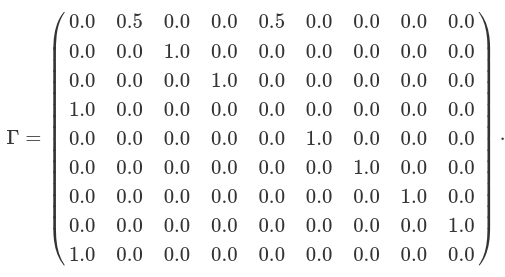
\includegraphics{Trabalho 03 - img4.png}

Esta cadeia é irredutível? ou seja, prove que o conjunto de estados
irredutíveis F satisfaz F=S, sendo S=\{1,⋯,9\}. Prove também que esta
cadeia é recorrente, ou seja, prove que cada estado em S é recorrente.

\textbf{Desenvolvimento:}

Verificando o \emph{summary} da cadeia:

\begin{verbatim}
Γ  Markov chain that is composed by: 
Closed classes: 
1 2 3 4 5 6 7 8 9 
Recurrent classes: 
{1,2,3,4,5,6,7,8,9}
Transient classes: 
NONE 
The Markov chain is irreducible 
The absorbing states are: NONE
\end{verbatim}

Aqui temos que todos os estados se comunicam, logo a matriz é
irredutível. Também observamos que os estados são ditos recorrentes.

Do teorema 17: Seja \textbf{F} um conjunto finito e fechado de estados
irredutíveis. Então cada estado em \textbf{F} é recorrente.

Como a matriz é irredutível e todos seus estados são recorrentes, a
matriz é dita recorrente.

\pagebreak

\hypertarget{exercicio-6---a-fiscaluxeda-de-muxeddia-identificou-seis-estados-associados-uxe0-televisuxe3o-0-nunca-assiste-tv-1-assiste-apenas-notuxedcias-2-assiste-tv-com-bastante-frequuxeancia-3-viciado-4-em-modificauxe7uxe3o-de-comportamento-5-morte-encefuxe1lica.-as-transiuxe7uxf5es-de-estado-para-estado-podem-ser-modeladas-como-uma-cadeia-de-markov-com-a-seguinte-matriz-de-transiuxe7uxe3o}{%
\subsection{Exercicio 6 - A Fiscalía de Mídia identificou seis estados
associados à televisão: 0 (nunca assiste TV), 1 (assiste apenas
notícias), 2 (assiste TV com bastante frequência), 3 (viciado), 4 (em
modificação de comportamento), 5 (morte encefálica). As transições de
estado para estado podem ser modeladas como uma cadeia de Markov com a
seguinte matriz de
transição:}\label{exercicio-6---a-fiscaluxeda-de-muxeddia-identificou-seis-estados-associados-uxe0-televisuxe3o-0-nunca-assiste-tv-1-assiste-apenas-notuxedcias-2-assiste-tv-com-bastante-frequuxeancia-3-viciado-4-em-modificauxe7uxe3o-de-comportamento-5-morte-encefuxe1lica.-as-transiuxe7uxf5es-de-estado-para-estado-podem-ser-modeladas-como-uma-cadeia-de-markov-com-a-seguinte-matriz-de-transiuxe7uxe3o}}

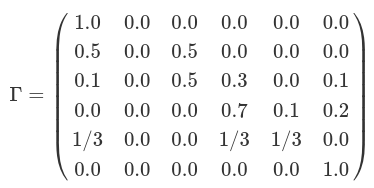
\includegraphics{Trabalho 03 - img6.png}

\begin{verbatim}
a) Quais estados são recorrentes e quais transientes.
b) Começando do estado $1$, qual é a probabilidade de o estado $5$ ser atingido antes do estado $0$, ou seja, qual é a probabilidade de um visualizador de notícias acabar com morte cerebral?
\end{verbatim}

\textbf{Desenvolvimento A:}

\begin{verbatim}
Γ  Markov chain that is composed by: 
Closed classes: 
0 
5 
Recurrent classes: 
{0},{5}
Transient classes: 
{1},{2},{3,4}
The Markov chain is not irreducible 
The absorbing states are: 0 5
\end{verbatim}

Pelo \emph{summary} da cadeia temos que os estados recorrentes (e
absorventes) são \{0\} e \{5\} e os transientes são \{1\}, \{2\},
\{3,4\}.

\pagebreak

\textbf{Desenvolvimento B:}

Para encontrarmos as probabilidades assintóticas, podemos utilizar uma
potência elevada da matriz de transição:

\begin{verbatim}
Γ^50000 
 A  6 - dimensional discrete Markov Chain defined by the following states: 
 0, 1, 2, 3, 4, 5 
 The transition matrix  (by rows)  is defined as follows: 
     0 1 2 3 4    5
0 1.00 0 0 0 0 0.00
1 0.66 0 0 0 0 0.34
2 0.32 0 0 0 0 0.68
3 0.20 0 0 0 0 0.80
4 0.60 0 0 0 0 0.40
5 0.00 0 0 0 0 1.00
\end{verbatim}

Logo, partindo do estado 1, o visualizador terá probabilidade de 0.34 de
ter morte cerebral antes de atingir o estado 0.

\end{document}
